%TCIDATA{LaTeXparent=0,0,relatorio.tex}
\begin{landscape}
\chapter{Diagramas simulink}\label{anexo:diagramas_simulink}
	
	\section{Simula��o}
	\begin{figure}[!hc]
		\centering
		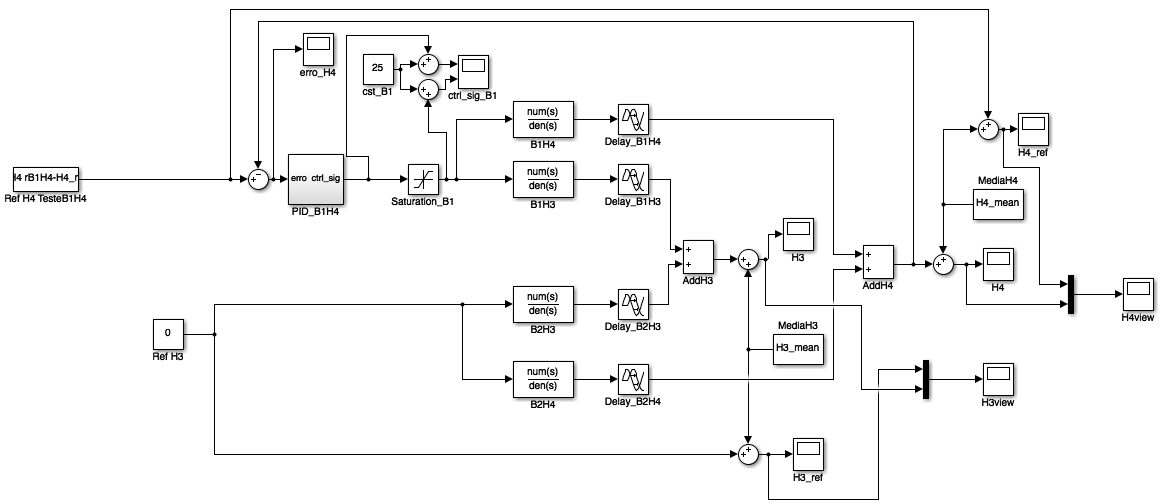
\includegraphics[scale=0.6]{figs/simulink_B1H4.png}
		\caption{Diagrama de simula��o para o PI $B_1H_4$}
	\end{figure}
	

%	\newpage
%	
%	\begin{figure}[!c]
%		\centering
%		\includegraphics[scale=0.6]{figs/simulink_H3H4.png}
%		\caption{Diagrama de simula��o para o PI $H_3H_4$}
%	\end{figure}
%	
	\newpage
	\FloatBarrier
	

	\section{Diagrama para aplica��o real}
	
	\begin{figure}[!ch]
		\centering
		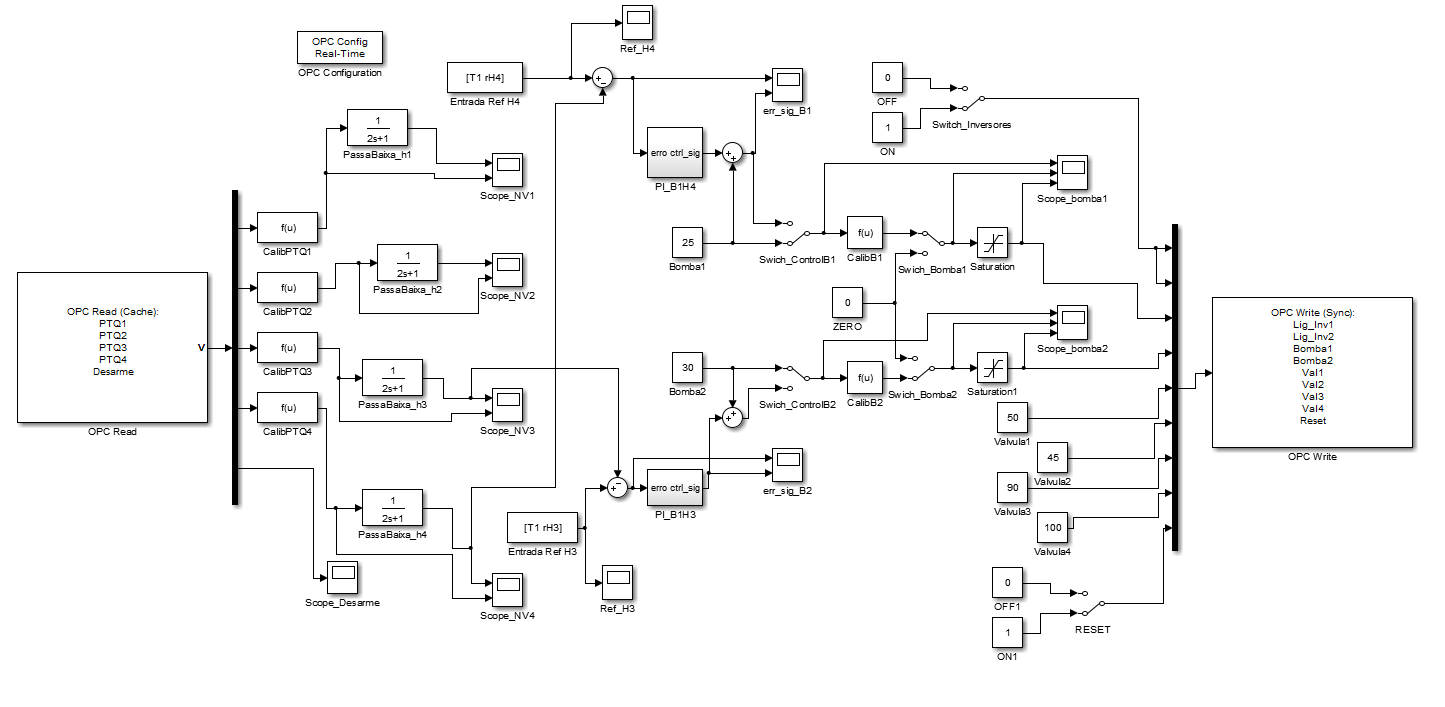
\includegraphics[scale=0.65]{figs/simulink_aplicacao_controle.png}
		\caption{Diagrama para aplica��o de controle na bancada e testes em malha aberta}
	\end{figure}
	

\end{landscape}